En este capítulo definiremos lo que es un proyecto de SmartRural usando diferentes definiciones, mostrando proyectos que están relacionados con el entorno del medio rural y comparandolas con nuestro proyecto.

\newpage

El término SmartRural surgió hace unos años como sinónimo del proyecto europeo Smart Village \cite{smart-village} (aldea inteligente), con el ánimo de añadir tecnologías TIC al mundo rural para optimizar el trabajo y por ende, aumentar la productividad y los beneficios al explotar los cultivos.

Respecto a esto último, solo queda añadir como dato que actualmente hay en total como unos 21 pueblos seleccionados en toda la Unión Europea (UE), para sumarse a este cambio digital y están supervisados por 28 expertos, uno por cada país miembro, y coordinados a nivel superior por E40 Group \cite{e40group} con socios como IfLS and empirica \cite{ifls} (Alemania), Innovatiesteunput \cite{innovatiesteunput} (Bélgica), Agricultural University of Athens \cite{greece} (Grecia) and eConcepts \cite{econcepts} (Irlanda).

A parte del proyecto europeo con subvención de la misma Unión Europea, existe un proyecto que merece especial atención y que se basa en mezclar tecnología informática con el medio rural. Este es Smart Rural \cite{smart-rural} (Agricultura Inteligente). 

Este proyecto, surgió en 2015 en Castilla y León, con la idea de mejorar mediante la tecnología, la Agricultura de Precisión. A parte, este proyecto contiene un sistema de gestión de recursos agrícolas y una bitacora para indicar que ha ido bien, que ha ido mal y posibles mantenimientos a realizar en distintas zonas.

Como dato a añadir a esto último, Smart Rural se ha convertido en una empresa respetable tanto dentro del sector de la tecnología, como del sector de la agricultura. Tiene presencia en países europeos y en países de hispanoamérica, como Chile o Argentina, y además ha recibido distintivos premios como ``Premio a la mejor empresa innovadora ADE2020'' (2015), ``Premio al emprendimiento por Aranda Emprende'' (2015), ``Premio Hermano Celestino'' (2016) y ``Premio a la innovación en Infoagro Exhibition'' (2019) \cite{team-smartrural}.

A continuación, en la Figura 2.1, se puede observar la página web principal de la empresa Smart Rural.

\begin{figure}[H]
    \centering
    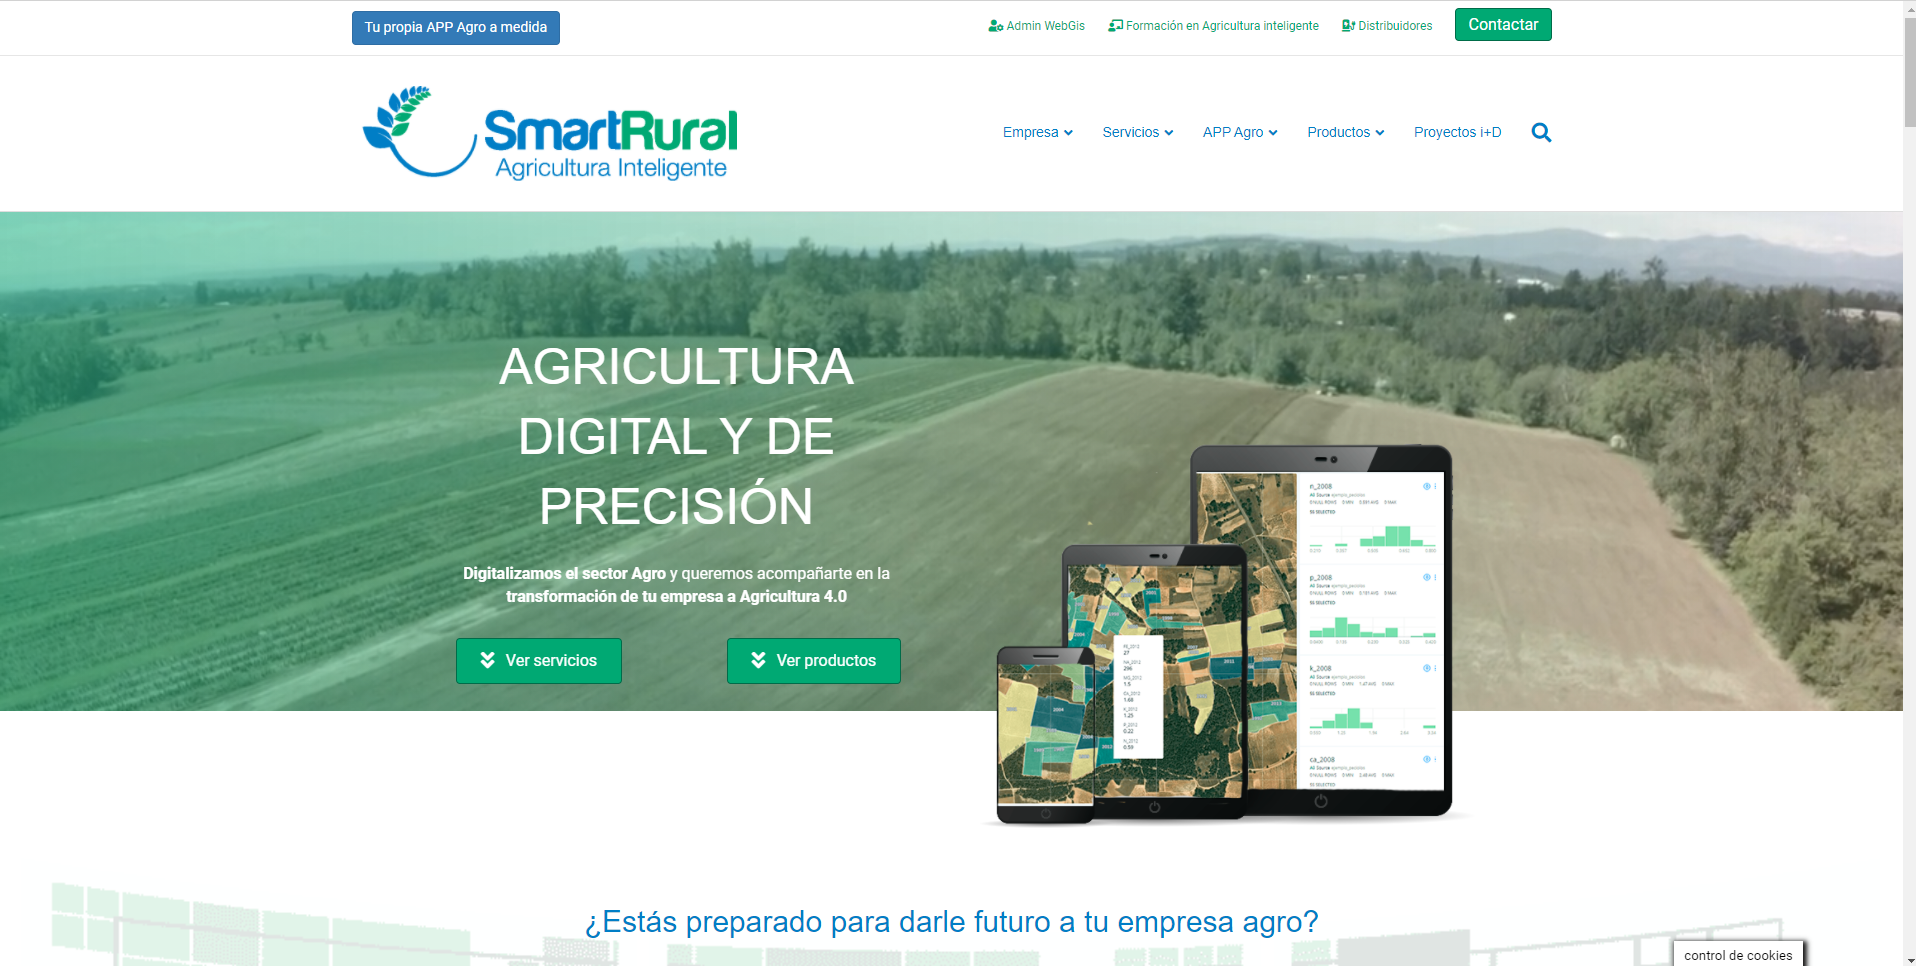
\includegraphics[width=0.85\linewidth]{images/state-art/smartrural.png}
    \caption{https://smartrural.net/}
\end{figure}

Nuestra aplicación tiene un ámbito parecida a la expuesta anteriormente, pero con un cambio significativo. Nuestro proyecto tendrá capacidad multiplataforma gracias al SDK de Ionic y Azure Cloud, además que añadimos un Sistema de IoT para detección de eventos, apostando por el desarrollo de aplicaciones híbridas y programación reactiva.

Además, ofrecemos almacenamiento online gracias a la perfecta integración que tienen estas tecnologías híbridas con las nubes de computación públicas existentes, tanto Azure Cloud para el procesamiento de datos como Amazon Web Services con su Relational Database Service para guardar los datos.

Por último, ofrecemos una tabla, Cuadro 2.1, con la comparativa entre el proyecto europeo, Smart Rural y nuestro proyecto, para identificar de forma breve y sencilla las diferencias entre la competencia y nosotros.

\begin{table}[!htbp]
    \centering
    \resizebox{\textwidth}{!}{
        \begin{tabular}{rlllrrrrr}
        \hline
            Características & Smart Village & Smart Rural & Nuestro proyecto \\
        \hline
            Integración Nube & No & No & Sí \\
            Aplicaciones Móviles & No & Sí & Sí \\
            Detección de Eventos & No & No & Sí \\
            Gestor de Recursos & No & Sí & Sí \\
            Interconectividad entre plataformas & Sí & Sí & Sí \\
            Sistema de IoT & No & No & Sí \\
            Sistemas de Gráficos y Estadísticas & Sí & Sí & No \\
            Sistema de Marketing Digital & No & Sí & No \\
        \hline
        \end{tabular}
    }
    \caption{Tabla comparativa}
\end{table}

